% -*- mode: LaTeX; coding: utf-8; -*-

\chapter{Web-palveluiden tulevaisuus}

Toimivan ja ennen kaikkea turvallisen web-pohjaisen palvelun tarjoaminen vaatii
nykyisin paljon enemmän huomiota ja aikaa niin palvelun kehittäjältä kuin myös
palvelun tarjoajalta ja ylläpitäjältä kuin ennen. Ajat ovat muuttuneet siitä,
jolloin käyttäjät selailivat pääasiassa staattisia web-sivuja, ja käyttivät
palveluista korkeintaan sähköpostia. Kehitys kulkee kovaa vauhtia eteenpäin, ja
tämän päivän suurimpia villityksiä ovat asiat kuten interaktiivisuus,
sosiaalisuus ja yksilöllisyys, joiden kautta verkon käytöstä pyritään tekemään
käyttäjälle entistä henkilökohtaisempi kokemus. Palvelut kuten MySpace,
Facebook ja YouTube ovat edelleen vahvistaneet näitä käyttäjätottumuksia, ja
markkinoille onkin syntynyt kova kilpailu siitä, kuka kehittää seuraavan
hittipalvelun. Nykyisin puhutaankin internetin seuraavasta evoluutiosta Web 2.0:
n muodossa, joita myös edellä mainitut palvelut edustavat. Uudet teknologiat ja
kiire tuovat kuitenkin aina mukanaan joukon uusia heikkouksia, joita hyökkääjät
pyrkivät hyödyntämään. Ylläpitäjien kannalta onkin tärkeää, että kehityksen
tuomiin haasteisiin pyritään vastaamaan mahdollisimman nopeasti ja tehokkaasti.

\section{Mitä tarkoittaa Web 2.0?}

Web 2.0 on termi, jota käytetään hyvin monessa eri tarkoituksessa ja
asiayhteydessä. Se yhdistetään usein mm. uuteen web-teknologiaan tai internet-
aikakauden tuotteen/palvelun kehityskaaren esittämiseen \cite{WEB2}. Yhteistä näille
on, että ne pyrkivät kuvaamaan sitä muutosta, jota internet pitää tällä
hetkellä sisällään. Tämä muutos on lähtöisin siitä, että kuluttajatottumukset
ovat kehittyneet kohti interaktiivisia palvelumalleja, joissa käyttäjillä on
suuri vaikutusvalta siihen mitä informaatiota esitetään ja kuinka se esitetään.
Sosiaalisuus ja sen luoma yhteisöllisyys ovat luoneet tarpeen palveluille,
joissa käyttäjät pystyvät tekemään useita asioita samaan aikaan saumattomasti
yhdestä paikasta käsin. Toinen kantava voima muutokselle on markkinoiden tuoma
paine, joka pyrkii mukautumaan muuttuneisiin vaatimuksiin sekä
kuluttajapuolella että yrityspuolella. Tätä varten joudutaan kehittämään yhä
isompia kokonaisuuksia uusilla teknologioilla, joiden käyttöä ei vielä hallita
tarpeeksi. Tähän kun vielä lisätään kiire päästä markkinoilla ensimmäisten
joukossa, niin tietoturva jää usein taka-alalle \cite{WEB2b}.

Tietoturvan kannalta teknologiat, jotka luetaan kuuluvan osaksi Web 2.0
teknologiaperhettä, ovat jatkuvan huomion kohteena. Nämä teknologiat
muodostavat sen voiman, joka mahdollistaa siirtymisen interaktiivisiin
sovelluksiin kuten Google Maps, ja yritysten toiminnan siirtymisen verkkoon.
Teknologiat kuten Asynchronous JavaScript (AJAX), Cascading Style Sheet (CSS),
Flash, ActiveX ja XML voidaan kaikki laskea kuuluvan osaksi Web 2.0-perhettä.
Osa näistä teknologioista on ollut jo pidemmän aikaa käytössä kun taas osaa on
vasta nyt alettu käyttämään siihen, mihin ne alun perin oli suunniteltu \cite{WEB2}.
Kuvassa \ref{web} on nähtävillä näiden yleisimpien teknologioiden ja protokollien
väliset suhteet.

\begin{figure}[htp]
\centering
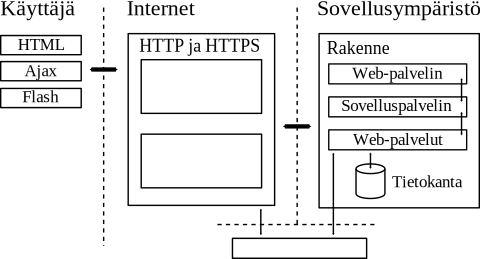
\includegraphics[width=12cm]{pics/web.pdf}
\caption{Web 2.0}
\label{web}
\end{figure}

Mitä Web 2.0 sitten tarkoittaa tietoturvan kannalta? Ensinnäkin sen mukana
tulee samat vanhat haavoittuvuudet kuin mitä Web 1.0 sisälsi. Näiden lisäksi
hyökkäykset kuten Cross-site Scripting (XSS) ja Cross-site Request Forgery (
CSRF) ovat aikaisempaa vaarallisia, koska käytetyt teknologiat mahdollistavat
rikkaamman ympäristön, jonka kautta murtautua järjestelmiin \cite{WEB2}. Web 2.0
sovellukset antavat myös loppukäyttäjälle ja takana oleville ohjelmille enemmän
valtaa, jonka johdosta loppukäyttäjä ei välttämättä edes huomaa joutuessaan
tietomurron kohteeksi. Otetaan esimerkiksi Ajax-teknologia, joka mahdollistaa
sivujen tietojen päivittämisen käyttäen asynkronisia kutsuja. Tämän ansiosta
käyttäjä pystyy tekemään kutsuja palvelimille ja päivittämään osan sivun
tiedoista niin, ettei koko sivua tarvitse päivittää. Tästä suurin osa tapahtuu
käyttäjältä piilossa, joten hän ei todennäköisesti huomaa, jos selain lataa
haitallisia ohjelmia koneelle käyttäen jotain tunnettua haavoittuvuutta.
Arviolta 70 prosenttia kaikista haitallisista koodeista ladataankin käyttäen
Ajaxia \cite{WEB2c}.

Palvelinpuolella muutokset eivät rajoitu vain Web 2.0 tuomiin
tietoturvariskeihin, sillä uudenlainen ajattelu vaatii myös uudenlaisen
palveluarkkitehtuurin. Uusi arkkitehtuuriratkaisu tuo aina mukanaan suuren
joukon muutoksia, jotka tulee ottaa huomioon tietoturvaa suunniteltaessa.
Palvelukeskeinen arkkitehtuuri (engl. Service Oriented Architecture, SOA) on
yksi näistä kehysmalleista, joka on kasvattanut kannatustaan Web 2.0:n
vanavedessä. SOA-arkkitehtuurilla onkin nykyisin tärkeä rooli palvelujen
välisen kommunikoinnin kehittämisessä. Siksi onkin tärkeää ymmärtää mistä
palasista SOA-arkkitehtuuriin perustuvat palvelut koostuvat, ja mitä tämä
tarkoittaa turvallisuuden kannalta.

\section{Palvelukeskeinen arkkitehtuuri}

Web-pohjaiset teknologiat ovat saamassa yhä suurempaa huomiota yrityspuolen
sovelluskehityksessä. Tätä muutosta on ollut ohjaamassa teknologioiden
kehittyminen siihen pisteeseen, jossa yritykset pystyvät tarjoamaan aikaisemmin
asiakas-serveri sovelluksia verkon välityksellä luotettavasti ja nopeasti. Tämä
ratkaisu on tuonut mukanaan rahallisia säästöjä yrityksille, jotka ovat ennen
joutuneet itse huolehtimaan mm. sovellusten ajan tasalla pitämisestä ja
palvelimien ylläpitämisestä \cite{WEB2}. Tämä muutos on luonut myös tarpeen löytää yhä
tehokkaampia kehitysmalleja ja tapoja toteuttaa entistä monimutkaisempia ja
vaativimpia sovelluksia suuryritysten tarpeisiin. Yksi tapa hallita tätä
muutosta on perustaa tehdyt ohjelmistosuunnitelman ratkaisut palvelukeskeisen
arkkitehtuurin malliin.

Puhuttaessa web-palveluista palvelukeskeinen arkkitehtuuri lähtee siitä
ajatuksesta, että palveluiden toiminnot ja prosessit pyritään suunnittelemaan
toimimaan mahdollisimman itsenäisesti ja avoimesti siten, että niitä pystytään
kutsumaan joustavasti eri sovellusten välillä käyttäen standardoitua rajapintaa.
Tähän ratkaisuun on ajanut pyrkimys laskea IT-kustannuksia ja maksimoida jo
käytössä olevien ratkaisujen uudelleenkäyttöä. Aikaisemmin tämän toteuttaminen
on ollut vaikeaa sovellusten heterogeenisyyden takia, jonka johdosta eri
alustojen ja toimittajien väliset yhteistoiminnot ovat olleet usein mahdottomia
toteuttaa. Yhä useamman sovelluksen ja palvelun siirtyessä verkkoon tästä
halutaan nyt päästä eroon, ja tähän ongelmaan palvelukeskeinen arkkitehtuuri
pyrkii tuomaan ratkaisun. Käytännössä tämä tarkoittaa sitä, että arkkitehtuurin
tulee tarjota sovelluksille mahdollisimman joustavan sekä sijainnista ja
protokollasta riippumattoman alustan \cite{SOA}. Tämän avulla loppukäyttäjälle
voidaan tarjota palveluita monesta eri paikasta yhtä aikaa siten, ettei hän ole
tästä edes tietoinen. Kyseessä on sama ajattelumalli johon Web 2.0 sovellukset
pohjautuvat, ja siksi palvelukeskeinen arkkitehtuuri onkin saanut paljon
nostetta Web 2.0:n myötä.

Palvelukeskeisen arkkitehtuurin tuomat edut eivät rajoitu pelkästään
kustannussäästöihin. Sen tuomiin etuihin kuuluu myös mm. uusien toimintojen
helpompi integrointi jo käytössä oleviin järjestelmiin sekä monimutkaisten
kokonaisuuksien helpompi hallinta. Organisaatiolle on myös tärkeää, että tällä
tavalla suunniteltuun palvelumalliin muutoksia on nopeampi tehdä ja reagointi
markkinamuutoksiin voidaan toteuttaa nopeassa aikataulussa \cite{WEB2c}. Tämä on
erityisen tärkeää, koska markkinoille on ilmestynyt monia uusia tekniikoita,
jotka mahdollistavat web-palveluiden integroinnin jo käytössä oleviin
palveluihin. Onkin arvioitu, että vuonna 2008 web-pohjaisiin palveluihin
käytettiin jo yli 11 miljardia dollaria, ja osa fokuksesta on jo siirtynyt
kohti keskikokoisia ja pieniä yrityksiä. Web-pohjaisten palveluiden merkityksen
uskotaankin entisestään kasvavan ja yritykset, jotka eivät reagoi tähän
muutokseen, huomaavat tulevaisuudessa olevansa epäsuotuisassa asemassa \cite{WEB2b}.

Palvelinpuolelle tapahtuva muutos tarkoittaa sopeutumista uudenlaiseen
ajattelumalliin, jossa palvelut on hajautettu ympäri verkkoa, ja joista osa ei
välttämättä ole saman ylläpitäjän hallinnassa. Kuvan \ref{soa} mukainen ratkaisu
tulee olemaan tulevaisuudessa arkipäivää, ja se tuo mukanaan uusia rajapintoja,
joiden kautta hyökkääjä voi pyrkiä murtautumaan järjestelmään tai jopa
yrityksen sisäiseen verkkoon. Koska palveluiden välinen kommunikointi perustuu
tässä mallissa luottamussuhteen luomiseen, tulee erityistä kiinnittää huomiota
siihen kuinka salaukset ja tunnistautuminen hoidetaan web-palveluita tarjoavien
osapuolien sekä käyttäjien kesken \cite{WEB2b}.

\begin{figure}[htp]
\centering
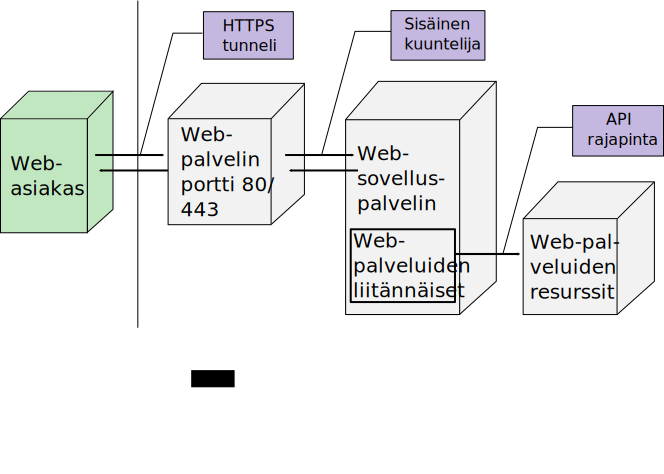
\includegraphics[width=12cm]{pics/soa.pdf}
\caption{SoA-arkkitehtuuri}
\label{soa}
\end{figure}

\section{Web-palveluiden tietoturva}

Internetin kehittyessä myös web-palveluihin kohdistuvat hyökkäykset ovat saaneet
uusia ilmenemismuotoja. Aikaisemmin ``web hakkerointia'' käytettiin kuvaamaan
hyökkäyksiä, jotka kohdistuivat palveluita tarjoaviin alustoihin kuten Apache, 
Microsoft IIS ja LAMP. Nämä hyökkäykset perustuivat tunnettujen haavoittuvaisuuksien
hyödyntämiseen, ja oikeille työkaluilla varustautunut hyökkääjä pystyikin kaatamaan haavoittuvan
palvelun muutamassa minuutissa. Esimerkiksi tunnetuimpien internet-matojen Code Redin ja Nimdan toiminta
perustui Microsoft IIS:sä olevan haavoittuvuuden hyödyntämiseen \cite{Hacking}. 

Tämänlaiset hyökkäykset ovat kuitenkin
menettäneet suurimman tehonsa, koska tehdyistä virheistä on opittu. Löydettyihin haavoittuvaisuuksiin
reagoidaan entistä nopeammin, yhä useampi alusta on konfiguroitu oikein ja saatavilla on työkaluja, joiden
avulla pystytään nopeasti ja helposti havaitsemaan yleisimmät tietoturvariskit \cite{Hacking}. Näistä seikoista johtuen
hyökkääjät ovatkin kiinnittäneet entistä enemmän huomiota itse alustalla pyöritettäviin palveluihin pyrkien 
murtautumaan järjestelmiin näiden kautta. Web 2.0:n myötä tämän tyyppiset hyökkäykset ovat saaneet entistä
enemmän huomiota, sillä se on tarjonnut hakkereille entistä monipuolisemman hyökkäyspinnan. Tietoturvan 
kannalta onkin tärkeää, että kumpaankin hyökkäystyyppiin kiinnitetään huomiota.

\subsection{Web-palvelimien turvaaminen}

Yllä mainitut seikat eivät tarkoita sitä, että web-palveluita pyörittävät alustat olisivat
turvassa hyökkäyksiltä. Onnistuneet hyökkäykset ovat edelleen yhtä tuhoisa, jos niihin ei ole ennalta 
varauduttu. Nämä erilaiset hyökkäykset pyrkivät yleensä hyödyntämään seuraavissa kategorioissa olevia heikkouksia

\begin{itemize}
\item Valmiit esimerkkitiedostot
\item Lähdekoodin paljastuminen
\item Kanonisointi
\item Palvelmiin asennetut lisäosat
\item Syötteen tarkistaminen \cite{Hacking}.
\end{itemize}

Näiltä suojautuminen on melko yksinkertaista, kunhan muistaa noudattaa muutamaa pääperiaatetta. Ensinnäkin tuotannossa 
olevilla palvelimilla ei tulisi koskaan olla asennettuna tai käytettynä tiedostoja, joiden turvallisuudesta ei ole
takeita. Näihin tiedostoihin kuuluvat mm. paketeissa mukana tulleet esimerkkitiedostot ja palvelimelle asennettavat 
lisäosat, joiden alkuperästä ei ole varmuutta. Toisekseen on tärkeää varmistaa, että käytettyihin sovelluksiin
on asennettu viimeisimmät päivitykset, sillä nämä yleensä korjaavat tunnetut heikkoudet \cite{Hacking}. Jo pelkästään näillä 
toimilla pystytään suurimmaksi osaksi estämään palvelmiin kohdistuvat hyökkäykset. 

\subsection{SQL injektio}

Virheelliseen syöttötietoon perustuvat hyökkäykset ovat jo pidemmän aikaa vaivanneet web-pohjaisia sovelluksia.
Web 2.0:n myötä hyökkäykset ovat entisestään yleistyneet, sillä monimutkaisten sovellusten takana käytetään entistä
enemmän erilaisia tietokantapohjaisia ratkaisuja kuten MySQL. Nämä hyökkäykset hyödyntävät sitä seikkaa, että suurin osa
sovelluksista ei tee selkeää eroa käyttäjän antaman syötteen ja ohjelmalle annettavien ohjeiden välillä. Tämä mahdollistaa
sen, että hyökkääjä pystyy piilottamaan annettuun hakuun ohjelmatason käskyjä, jotka muokkaavat sovelluksen toimintaa
hyökkääjän haluamaan suuntaan \cite{WEB2}. Normaaleilla toimenpiteillä tällaisen hyökkäysten tunnistaminen on hankalaa, sillä
yritysten tietoturvasta vastaavat palomuurit toimivat OSI-mallin kolmannella, neljännellä ja viidennellä kerroksella, eivätkä ne tunnista
ylimmän tason eli ohjelmistotason kautta tulevia hyökkäyksiä. Tämän lisäksi useimmat palomuurit eivät ymmärrä protokollien
kuten HTTP:n tarkkaa sisältöä \cite{SQL SS}.    

Onnistunut injektiohyökkäys koostuu kolmesta erillisestä vaiheesta. Ensimmäisessaä vaiheessa hyökkääjän tulee tunnistaa 
web-sovelluksessa käytetyt teknologiat. Tämä onnistuu mm. tulkitsemalla sivujen antamia virheilmoituksia, tutkimalla 
sivun lähdekoodia tai käyttäen tätä varten tehtyjä työkaluja kuten Nessus ja Nmap. Tämä vaihe on hyökkääjälle melko triviaali
tehtävä, mutta hyökkäyksen kannalta tiedot ovat elintärkeitä, sillä injektiohyökkäyksen onnistuminen on täysin riippuvainen 
käytetystä ohjelmointikielestä. Kun tarvittavat tiedot on saatu kerättyä, voidaan varsinaista hyökkäystä alkaa suunnittelemaan.
Tämä tapahtuu tunnistamalla ne syötteet, jotka käyttäjä pystyy sovellukselle antamaan. Tämä käsittää käytännössä kaiken sen 
datan, joka kulkee HTTP GET ja HTTP POST pyynnöissä. Viimeisessä vaiheessa hyökkääjän tehtäväksi jää sitten niiden syötteiden 
tunnistaminen, joita käyttämällä sovelluksen toiminta saadaaan muokattua. Tähänkin tehtävään löytyy useita työkaluja, ja
monessa tapauksessa samat periaatteet toimivat eri sovellusten välillä \cite{WEB2}.

Structured Query Language (lyh. SQL), joka on alan de facto standardi tietokantojen käsittelyyn, on käytössä lähes jokaisessa
web-sovelluksessa, joka käyttää jonkinlaista tietokantaratkaisua. Sen syntaksi on sekoitus ohjelmakäskyjä ja käyttäjän antamia
syötteitä, ja huonosti määritettynä käyttäjän antama syöte voidaan tulkita virheellisesti ohjelmatason käskyksi. Tämän syötteen
hyökkääjä joutuu usein etsimään sokeasti, mutta syötteet kuten

\begin{itemize}
\item ' OR 1=1 "{-}{-}
\item ') OR 1=1 "{-}{-}
\end {itemize}
\linebreak
toimivat hyvin usein \cite{WEB2}. Virheellisestä hausta aiheutuvat virheilmoitukset antavat myös erittäin paljon
hyödyllistä tietoa hyökkääjälle \cite{SQL SS}. Koska suurin osa SQL-tietokannoista mahdollistaa useamman perättäisen syötteen 
antamisen, kunhan syntaksi pysyy oikeana, voidaan näiden avulla katkaista ohjelman normaali toiminta. Otetaan esimerkiksi SQL-haku
\begin{center}\tt
String query= ``SELECT id FROM user\_table WHERE `` + \\
``username = ' `` + username + ``' AND `` + \\
``password = PASSWORD(' `` + password + ``')''; \\
\end{center}
\end{tt}
\linebreak
Antamalla käyttäjänimeksi arvon

\begin{center}\tt
' OR 1=1; DROP TABLE user\_table;"{-}{-}
\end{center}
\end{tt}
\linebreak
muuttuu tietokannalle ohjautuva kysely muotoon

\begin{center}\tt
String query= ``SELECT id FROM user\_table WHERE username=' ' OR 1=1; DROP TABLE
user\_table; "{-}{-} ' AND password = PASSWORD ('x');
\end{center}
\end{tt}
\linebreak
SQL-kielessä kaksi perättäistä viivaa tarkoittaa, että kaikki siitä oikealla puolella oleva on kommenttia. 
Näin ollen lopullinen SQL-haku on 

\begin{center}\tt
String query= ``SELECT id FROM user\_table WHERE \\username=' ' OR 1=1; DROP TABLE
user\_table;
\end{center}
\end{tt}
\linebreak
Näin muodostettu haku on syntaktisesti täysin oikea, ja se tyhjentää tietokannassa olevan user\_table tiedoston, joka pitää
sisällään järjestelmään tallennetut käyttäjät \cite{WEB2}. 

Vastaavanlaisia tekniikoita käyttäen hyökkääjä pystyy tekemään kaiken sen, joka pystytään esittämään SQL-kyselynä, ja johon ajettavalla
sovelluksella on riittävät oikeudet. Mielivaltaisten käskyjen antaminen, DLL tiedostojen luominen ja ajaminen ja tietokannan
sisällön lähettäminen jollekin toiselle internetissä olevalle palvelimelle ovat vain muutamia esimerkkejä toiminnoista, joita
onnistunut hyökkäys voi aiheuttaa \cite{SQL SS}.

Injektiohyökkäykset eivät rajoitu pelkästään SQL-kieleen, sillä useat eri tekniikat kuten XPath ja LDAP sisältävät vastaavanlaisia heikkouksia.
SQL-kieleen pohjautuvat hyökkäykset ovat kuitenkin kaikista yleisimpiä johtuen SQL-kielen levinneisyydestä. 


\section{Työkaluja}
Palvelimien tietoturvasta vastaaminen on tarkkuuta ja aikaa vaativaa työtä. Se edellyttää jatkuvaa omien tietojen
päivittämistä sekä liikenteen ja palveluiden seuraamista. Jo pelkästään yleisimpien tietoturvariskien tunnistaminen ja
niiden korjaaminen käsin osoittautuu usein ylivoimaiseksi tehtäväksi varsinkin, jos ylläpidettävänä on monimutkaisia
ratkaisuja. Asian helpottamiseksi on onneksi saatavilla useita erilaisia työkaluja, jotka etsivät automaattisesti
tunnetuimpia tietoturva-aukkoja, ja suosittelevat keinoja kuinka nämä voidaan korjata. Samat työkalut ovat myös 
hakkereien käytössä, kun he etsivät heikkouksia joiden kautta murtautua järjestelmään. Siksi onkin tärkeää pyrkiä
korjaamaan löydetyt heikkoudet mahdollisimman pian, sillä sekä ylläpitäjillä että hyökkääjillä on samat tiedot saatavilla. 




